% Options for packages loaded elsewhere
\PassOptionsToPackage{unicode}{hyperref}
\PassOptionsToPackage{hyphens}{url}
\PassOptionsToPackage{dvipsnames,svgnames,x11names}{xcolor}
%
\documentclass[
  letterpaper,
  DIV=11,
  numbers=noendperiod]{scrreprt}

\usepackage{amsmath,amssymb}
\usepackage{iftex}
\ifPDFTeX
  \usepackage[T1]{fontenc}
  \usepackage[utf8]{inputenc}
  \usepackage{textcomp} % provide euro and other symbols
\else % if luatex or xetex
  \usepackage{unicode-math}
  \defaultfontfeatures{Scale=MatchLowercase}
  \defaultfontfeatures[\rmfamily]{Ligatures=TeX,Scale=1}
\fi
\usepackage{lmodern}
\ifPDFTeX\else  
    % xetex/luatex font selection
\fi
% Use upquote if available, for straight quotes in verbatim environments
\IfFileExists{upquote.sty}{\usepackage{upquote}}{}
\IfFileExists{microtype.sty}{% use microtype if available
  \usepackage[]{microtype}
  \UseMicrotypeSet[protrusion]{basicmath} % disable protrusion for tt fonts
}{}
\makeatletter
\@ifundefined{KOMAClassName}{% if non-KOMA class
  \IfFileExists{parskip.sty}{%
    \usepackage{parskip}
  }{% else
    \setlength{\parindent}{0pt}
    \setlength{\parskip}{6pt plus 2pt minus 1pt}}
}{% if KOMA class
  \KOMAoptions{parskip=half}}
\makeatother
\usepackage{xcolor}
\setlength{\emergencystretch}{3em} % prevent overfull lines
\setcounter{secnumdepth}{5}
% Make \paragraph and \subparagraph free-standing
\makeatletter
\ifx\paragraph\undefined\else
  \let\oldparagraph\paragraph
  \renewcommand{\paragraph}{
    \@ifstar
      \xxxParagraphStar
      \xxxParagraphNoStar
  }
  \newcommand{\xxxParagraphStar}[1]{\oldparagraph*{#1}\mbox{}}
  \newcommand{\xxxParagraphNoStar}[1]{\oldparagraph{#1}\mbox{}}
\fi
\ifx\subparagraph\undefined\else
  \let\oldsubparagraph\subparagraph
  \renewcommand{\subparagraph}{
    \@ifstar
      \xxxSubParagraphStar
      \xxxSubParagraphNoStar
  }
  \newcommand{\xxxSubParagraphStar}[1]{\oldsubparagraph*{#1}\mbox{}}
  \newcommand{\xxxSubParagraphNoStar}[1]{\oldsubparagraph{#1}\mbox{}}
\fi
\makeatother

\usepackage{color}
\usepackage{fancyvrb}
\newcommand{\VerbBar}{|}
\newcommand{\VERB}{\Verb[commandchars=\\\{\}]}
\DefineVerbatimEnvironment{Highlighting}{Verbatim}{commandchars=\\\{\}}
% Add ',fontsize=\small' for more characters per line
\usepackage{framed}
\definecolor{shadecolor}{RGB}{241,243,245}
\newenvironment{Shaded}{\begin{snugshade}}{\end{snugshade}}
\newcommand{\AlertTok}[1]{\textcolor[rgb]{0.68,0.00,0.00}{#1}}
\newcommand{\AnnotationTok}[1]{\textcolor[rgb]{0.37,0.37,0.37}{#1}}
\newcommand{\AttributeTok}[1]{\textcolor[rgb]{0.40,0.45,0.13}{#1}}
\newcommand{\BaseNTok}[1]{\textcolor[rgb]{0.68,0.00,0.00}{#1}}
\newcommand{\BuiltInTok}[1]{\textcolor[rgb]{0.00,0.23,0.31}{#1}}
\newcommand{\CharTok}[1]{\textcolor[rgb]{0.13,0.47,0.30}{#1}}
\newcommand{\CommentTok}[1]{\textcolor[rgb]{0.37,0.37,0.37}{#1}}
\newcommand{\CommentVarTok}[1]{\textcolor[rgb]{0.37,0.37,0.37}{\textit{#1}}}
\newcommand{\ConstantTok}[1]{\textcolor[rgb]{0.56,0.35,0.01}{#1}}
\newcommand{\ControlFlowTok}[1]{\textcolor[rgb]{0.00,0.23,0.31}{\textbf{#1}}}
\newcommand{\DataTypeTok}[1]{\textcolor[rgb]{0.68,0.00,0.00}{#1}}
\newcommand{\DecValTok}[1]{\textcolor[rgb]{0.68,0.00,0.00}{#1}}
\newcommand{\DocumentationTok}[1]{\textcolor[rgb]{0.37,0.37,0.37}{\textit{#1}}}
\newcommand{\ErrorTok}[1]{\textcolor[rgb]{0.68,0.00,0.00}{#1}}
\newcommand{\ExtensionTok}[1]{\textcolor[rgb]{0.00,0.23,0.31}{#1}}
\newcommand{\FloatTok}[1]{\textcolor[rgb]{0.68,0.00,0.00}{#1}}
\newcommand{\FunctionTok}[1]{\textcolor[rgb]{0.28,0.35,0.67}{#1}}
\newcommand{\ImportTok}[1]{\textcolor[rgb]{0.00,0.46,0.62}{#1}}
\newcommand{\InformationTok}[1]{\textcolor[rgb]{0.37,0.37,0.37}{#1}}
\newcommand{\KeywordTok}[1]{\textcolor[rgb]{0.00,0.23,0.31}{\textbf{#1}}}
\newcommand{\NormalTok}[1]{\textcolor[rgb]{0.00,0.23,0.31}{#1}}
\newcommand{\OperatorTok}[1]{\textcolor[rgb]{0.37,0.37,0.37}{#1}}
\newcommand{\OtherTok}[1]{\textcolor[rgb]{0.00,0.23,0.31}{#1}}
\newcommand{\PreprocessorTok}[1]{\textcolor[rgb]{0.68,0.00,0.00}{#1}}
\newcommand{\RegionMarkerTok}[1]{\textcolor[rgb]{0.00,0.23,0.31}{#1}}
\newcommand{\SpecialCharTok}[1]{\textcolor[rgb]{0.37,0.37,0.37}{#1}}
\newcommand{\SpecialStringTok}[1]{\textcolor[rgb]{0.13,0.47,0.30}{#1}}
\newcommand{\StringTok}[1]{\textcolor[rgb]{0.13,0.47,0.30}{#1}}
\newcommand{\VariableTok}[1]{\textcolor[rgb]{0.07,0.07,0.07}{#1}}
\newcommand{\VerbatimStringTok}[1]{\textcolor[rgb]{0.13,0.47,0.30}{#1}}
\newcommand{\WarningTok}[1]{\textcolor[rgb]{0.37,0.37,0.37}{\textit{#1}}}

\providecommand{\tightlist}{%
  \setlength{\itemsep}{0pt}\setlength{\parskip}{0pt}}\usepackage{longtable,booktabs,array}
\usepackage{calc} % for calculating minipage widths
% Correct order of tables after \paragraph or \subparagraph
\usepackage{etoolbox}
\makeatletter
\patchcmd\longtable{\par}{\if@noskipsec\mbox{}\fi\par}{}{}
\makeatother
% Allow footnotes in longtable head/foot
\IfFileExists{footnotehyper.sty}{\usepackage{footnotehyper}}{\usepackage{footnote}}
\makesavenoteenv{longtable}
\usepackage{graphicx}
\makeatletter
\newsavebox\pandoc@box
\newcommand*\pandocbounded[1]{% scales image to fit in text height/width
  \sbox\pandoc@box{#1}%
  \Gscale@div\@tempa{\textheight}{\dimexpr\ht\pandoc@box+\dp\pandoc@box\relax}%
  \Gscale@div\@tempb{\linewidth}{\wd\pandoc@box}%
  \ifdim\@tempb\p@<\@tempa\p@\let\@tempa\@tempb\fi% select the smaller of both
  \ifdim\@tempa\p@<\p@\scalebox{\@tempa}{\usebox\pandoc@box}%
  \else\usebox{\pandoc@box}%
  \fi%
}
% Set default figure placement to htbp
\def\fps@figure{htbp}
\makeatother

\KOMAoption{captions}{tableheading}
\makeatletter
\@ifpackageloaded{tcolorbox}{}{\usepackage[skins,breakable]{tcolorbox}}
\@ifpackageloaded{fontawesome5}{}{\usepackage{fontawesome5}}
\definecolor{quarto-callout-color}{HTML}{909090}
\definecolor{quarto-callout-note-color}{HTML}{0758E5}
\definecolor{quarto-callout-important-color}{HTML}{CC1914}
\definecolor{quarto-callout-warning-color}{HTML}{EB9113}
\definecolor{quarto-callout-tip-color}{HTML}{00A047}
\definecolor{quarto-callout-caution-color}{HTML}{FC5300}
\definecolor{quarto-callout-color-frame}{HTML}{acacac}
\definecolor{quarto-callout-note-color-frame}{HTML}{4582ec}
\definecolor{quarto-callout-important-color-frame}{HTML}{d9534f}
\definecolor{quarto-callout-warning-color-frame}{HTML}{f0ad4e}
\definecolor{quarto-callout-tip-color-frame}{HTML}{02b875}
\definecolor{quarto-callout-caution-color-frame}{HTML}{fd7e14}
\makeatother
\makeatletter
\@ifpackageloaded{bookmark}{}{\usepackage{bookmark}}
\makeatother
\makeatletter
\@ifpackageloaded{caption}{}{\usepackage{caption}}
\AtBeginDocument{%
\ifdefined\contentsname
  \renewcommand*\contentsname{Table of contents}
\else
  \newcommand\contentsname{Table of contents}
\fi
\ifdefined\listfigurename
  \renewcommand*\listfigurename{List of Figures}
\else
  \newcommand\listfigurename{List of Figures}
\fi
\ifdefined\listtablename
  \renewcommand*\listtablename{List of Tables}
\else
  \newcommand\listtablename{List of Tables}
\fi
\ifdefined\figurename
  \renewcommand*\figurename{Figure}
\else
  \newcommand\figurename{Figure}
\fi
\ifdefined\tablename
  \renewcommand*\tablename{Table}
\else
  \newcommand\tablename{Table}
\fi
}
\@ifpackageloaded{float}{}{\usepackage{float}}
\floatstyle{ruled}
\@ifundefined{c@chapter}{\newfloat{codelisting}{h}{lop}}{\newfloat{codelisting}{h}{lop}[chapter]}
\floatname{codelisting}{Listing}
\newcommand*\listoflistings{\listof{codelisting}{List of Listings}}
\makeatother
\makeatletter
\makeatother
\makeatletter
\@ifpackageloaded{caption}{}{\usepackage{caption}}
\@ifpackageloaded{subcaption}{}{\usepackage{subcaption}}
\makeatother

\usepackage{bookmark}

\IfFileExists{xurl.sty}{\usepackage{xurl}}{} % add URL line breaks if available
\urlstyle{same} % disable monospaced font for URLs
\hypersetup{
  pdftitle={Introduction to R},
  pdfauthor={Daulton Selke},
  colorlinks=true,
  linkcolor={blue},
  filecolor={Maroon},
  citecolor={Blue},
  urlcolor={Blue},
  pdfcreator={LaTeX via pandoc}}


\title{Introduction to R}
\usepackage{etoolbox}
\makeatletter
\providecommand{\subtitle}[1]{% add subtitle to \maketitle
  \apptocmd{\@title}{\par {\large #1 \par}}{}{}
}
\makeatother
\subtitle{SOC 300: Social Research Methods}
\author{Daulton Selke}
\date{2025-09-03}

\begin{document}
\maketitle

\renewcommand*\contentsname{Table of contents}
{
\hypersetup{linkcolor=}
\setcounter{tocdepth}{2}
\tableofcontents
}

\bookmarksetup{startatroot}

\chapter*{Preface}\label{preface}
\addcontentsline{toc}{chapter}{Preface}

\markboth{Preface}{Preface}

Welcome to this introductory R tutorial for SOC 300!

Here you will find all the step-by-step instructions for completing our
initial foray into R for quantitative analysis of social science data.
We will begin by establishing some common ground in basic R operations
and functionality. After we lay this foundation, we will progress
through various data processing tasks---from importing and cleaning
public data to visualizing and analyzing these data for consumption by
interested stakeholders.

You will receive an R script file with the commands detailed here, so
that you can easily run and manipulate them on your own device, but you
will always be able to refer to this mini-textbook in the event that you
would like to see everything in one place and refer to some more
detailed documentation on various R operations.

\part{Day 1: Getting Started}

\chapter{Background}\label{background}

Before we start exploring some of R's basic functionality, I'm going to
set the stage a little on what R and R studio are, why we are using
these tools in particular, and what we will need to know before we dig
in.

\section{What is R?}\label{what-is-r}

At it's core, R is a programming language. There's a lot to say about
this from a computer science perspective, but, for our purposes, you can
just think of R as a language with a very particular structure that's
designed to tell our computers what to do.

There are all sorts of different programming languages out there, and
they all offer certain benefits or cater to particular computing needs.
Unlike some general purpose languages like C, C++, or Python, R is
relatively specialized, and this is part of what makes it so useful for
us. R is designed with statistical computing as a primary motivator, and
now---roughly 30 years into its tenure---stands as one of the most
widely adopted resources for statistical data science in the social
sciences and beyond.

Though there can be a bit of a learning curve when getting used to R, we
will focus on exactly the things that we need and build ourselves up
slowly. Once you get used to it, R will allow you to perform incredibly
complex statistical procedures with relative ease, and it can even help
us with other related tasks like visualizing and presenting our
analyses.

\section{What is R Studio?}\label{what-is-r-studio}

We are going to pair R with the software R Studio, which is what's known
as an Integrated Development Environment (IDE). Programming languages
can be leveraged in a number of different ways. You could run R commands
entirely from a Windows command line or Mac terminal. But that would
probably not be very ideal for us---not to mention sort of ethereal and
frustrating for those of without any programming experience. IDEs
provide user-friendly interfaces for working with programming languages,
so that we can easily manage our code, quickly generate and view the
output of our analyses, and generally keep track of what we are doing
with R. There are lots of other IDEs out there, but R Studio is an ideal
balance of ease and power, so it will serve as our IDE of choice.

The best way to think about R Studio's relationship to R is by framing
it as an analogy with a desktop computer. R Studio is to R as a monitor
is to a computer. R is the thing that's doing all the heavy lifting
computationally, and R Studio is the thing that allows us to view and
interact with R in a way that's simple and straightforward.

\section{Acquiring R and R Studio}\label{acquiring-r-and-r-studio}

All of the CHASS computers (and likely most NC State computers) come
with R and R Studio, so you do not need to download them, but you may
find it convenient to work on R assignments using your own personal
device, so I've provided some instructions below.

Note that you will want to install R first,

\subsection{Downloading R}\label{downloading-r}

You can download R from the
\href{https://www.r-project.org/}{Comprehensive R Archive Network
(CRAN)}.

When you click that link, you will arrive at CRAN's homepage. Navigate
to the sidebar on the left, find `Download' near the top, and then click
`CRAN'. This will take you to the `mirrors' page. Mirrors are just
different host locations for downloading the R installation files. This
allows you to maximize download speed by choosing a nearby server, so
scroll down to `USA' and choose one of those (I usually opt for the
Durham, NC mirror).

Unless you are very experienced with computers, you should download one
of the options listed as `pre-compiled binary distributions'. These will
typically be the first options listed. Don't even worry about what that
means if you're not familiar. Just choose the one that reflects your
operating system (there are options for Windows, Mac, and Linux) That
should download an R installer, and you can follow the directions to
complete a default installation.

\subsection{Downloading R Studio}\label{downloading-r-studio}

R Studio is a little more straightforward to download. Just
\href{https://posit.co/download/rstudio-desktop/}{navigate to its
homepage}, scroll down a little, and you will find a big button that
says `Download R Studio for {[}your operating system{]}'. Go ahead and
run the installer with the default settings.

\chapter{R Fundamentals}\label{r-fundamentals}

In this first section, we are going to start from the ground up and
start to familiarize ourselves with the way R works and what it expects
from us. We will begin with the most basic building blocks of R data and
work our way up to the data frame---the object that will be most
relevant for us. While you won't generally need to build data frames
from scratch within R for your own research, it's a good way to
familiarize yourself with the structure of data in R. While we will
start here with a rather simple data frame, all the principles you learn
here will scale up as we start to work with much larger and more complex
data frames.

\begin{tcolorbox}[enhanced jigsaw, colback=white, title=\textcolor{quarto-callout-note-color}{\faInfo}\hspace{0.5em}{Note}, coltitle=black, bottomrule=.15mm, breakable, opacityback=0, colframe=quarto-callout-note-color-frame, leftrule=.75mm, opacitybacktitle=0.6, arc=.35mm, rightrule=.15mm, bottomtitle=1mm, toptitle=1mm, titlerule=0mm, toprule=.15mm, left=2mm, colbacktitle=quarto-callout-note-color!10!white]

I'm writing this mini-book in a language called
\href{https://quarto.org/}{Quarto}, which allows us to carry out a bunch
of neat formatting tasks with little effort. One of the big perks is
that Quarto can read and process R code, so I will show you all my R
code here, and you will be able to directly view the output. If you want
to follow along with your own script on your personal device, you should
copy and paste the commands from this document and run them locally.

\end{tcolorbox}

\section{Basic Operations}\label{basic-operations}

First, we will start by exploring some of the basic characteristics of
R.

R can be used as a simple calculator and will process both numbers and
conventional mathematical operator symbols. You can run the commands
below by placing your cursor at the beginning or end of the line and
pressing CTRL+Enter (Windows) or Command+Return (Mac)

\begin{Shaded}
\begin{Highlighting}[]
\DecValTok{5}\SpecialCharTok{+}\DecValTok{2}
\end{Highlighting}
\end{Shaded}

\begin{verbatim}
[1] 7
\end{verbatim}

You should see the result displayed in the console below.

\section{Storing Objects}\label{storing-objects}

R is especially helpful for allowing us to create and store objects that
we can call and manipulate later. We can create names for these objects
and then use R's `assignment operator,' the \texttt{\textless{}-}
symbol, to assign a value to our specified object name. Here, we'll
assign the previous calculation to an object that we are calling
\texttt{our\_object}.

If you run this command on your own device, you should see
\texttt{our\_object} populate in the upper-right Environment window.
This is where you can find all of the objects that you create in your R
session. We can run the object itself, as well as combine it with other
operations

\begin{Shaded}
\begin{Highlighting}[]
\NormalTok{our\_object }\OtherTok{\textless{}{-}} \DecValTok{5}\SpecialCharTok{+}\DecValTok{2}
\end{Highlighting}
\end{Shaded}

There are some more baroque ways around this, but it's best to operate
under the impression that object names cannot include spaces (or start
with numbers). This kind of thing is common in some programming
languages, so there are a couple stylistic conventions to address this.
I tend to use what's called `snake case,' which involves replacing
spaces with underscores. There's also `camel case,' where each word has
the first letter capitalized, e.g.~MyVariableName. I would settle on one
that you like and be consistent with it.

\begin{Shaded}
\begin{Highlighting}[]
\NormalTok{our\_object}
\end{Highlighting}
\end{Shaded}

\begin{verbatim}
[1] 7
\end{verbatim}

\begin{Shaded}
\begin{Highlighting}[]
\NormalTok{our\_object }\SpecialCharTok{+} \DecValTok{3}
\end{Highlighting}
\end{Shaded}

\begin{verbatim}
[1] 10
\end{verbatim}

\begin{Shaded}
\begin{Highlighting}[]
\NormalTok{our\_object }\SpecialCharTok{*} \DecValTok{100}
\end{Highlighting}
\end{Shaded}

\begin{verbatim}
[1] 700
\end{verbatim}

\section{A Note on Functions}\label{a-note-on-functions}

R is also useful for its implementation of functions, which you can
think of in the sense you likely learned in your math classes. Functions
are defined procedures that take some input value, transform that value
according to the procedure, and then output a new value.

R comes with a great deal of already defined functions, and we can use
these to perform all sorts of helpful operations. You can call a
function by indicating it's common name and then placing it's required
inputs between parentheses, e.g.~\texttt{function\_name(input)}.Note
that function inputs are also often referred to as `arguments'. We'll
get a lot of mileage out of functions, and part of the initial learning
curve of R will be related to getting used to the range of available
functions and the syntax you must follow to call them.

Now, let's take a step back and think about some of our basic building
blocks in R.

\section{Vectors and R Data Types}\label{vectors-and-r-data-types}

You can think of vectors as ordered sets of values. We can use the
\texttt{c()} function (short for `combine') to create a vector made up
of the values we provide. Let's make a few different vectors---each one
will have 5 separate items in it, and we separate those items with
commas. Note that when we want R to process something as text (and not a
named object, number, or function), we put it in quotation marks.

\begin{Shaded}
\begin{Highlighting}[]
\NormalTok{num\_vec }\OtherTok{\textless{}{-}} \FunctionTok{c}\NormalTok{(}\FloatTok{1.2}\NormalTok{, }\FloatTok{3.4}\NormalTok{, }\FloatTok{5.6}\NormalTok{, }\FloatTok{7.1}\NormalTok{, }\FloatTok{2.8}\NormalTok{)}

\NormalTok{character\_vec }\OtherTok{\textless{}{-}} \FunctionTok{c}\NormalTok{(}\StringTok{"east"}\NormalTok{, }\StringTok{"west"}\NormalTok{, }\StringTok{"south"}\NormalTok{, }\StringTok{"south"}\NormalTok{, }\StringTok{"north"}\NormalTok{) }

\NormalTok{logical\_vec }\OtherTok{\textless{}{-}} \FunctionTok{c}\NormalTok{(}\ConstantTok{TRUE}\NormalTok{, }\ConstantTok{FALSE}\NormalTok{, }\ConstantTok{TRUE}\NormalTok{, }\ConstantTok{FALSE}\NormalTok{, }\ConstantTok{FALSE}\NormalTok{) }
\end{Highlighting}
\end{Shaded}

Let's talk a bit about what we have here. Each of these vectors
represents a \textbf{data type} in R, or, in other words, one of the
basic ways in which R stores data. There are some more data types out
there, but these are the most most relevant for us.

\begin{itemize}
\item
  \textbf{\emph{Numeric Data:}} As the name suggests, this is the
  typical fashion in which numbers are stored in R. Numeric data
  encompasses both \emph{continuous} values and \emph{discrete} values.
  These are essentially numbers that can have decimal places
  vs.~integers (whole numbers).
\item
  \textbf{\emph{Character Data:}} Character here refers to the idea of
  character strings. This is typically how R stores text data---as
  distinct strings of text. Note that, while numbers are typically
  processed as numeric by R, numbers can also become character data if
  you place them between quotation marks.
\item
  \textbf{\emph{Logical Data:}} In R syntax, upper-case `true' and
  `false' have fixed values and, when used without quotes, will refer to
  these pre-defined logical values. We probably won't use this data type
  much for analyses, but we will run into them in other places. They can
  be useful for sorting and searching through subsets of data, and we
  will also use logical values to turn certain procedures on or off in
  some functions.
\end{itemize}

Many R functions will respond differently to different data types, so
it's important to keep these in mind when you need to troubleshoot
errors.

Take the \texttt{mean()} function, for example. As the name implies,
this function will return the arithmetic mean of a numeric vector. Let's
give it the one we just made above:

\begin{Shaded}
\begin{Highlighting}[]
\FunctionTok{mean}\NormalTok{(num\_vec)}
\end{Highlighting}
\end{Shaded}

\begin{verbatim}
[1] 4.02
\end{verbatim}

\begin{Shaded}
\begin{Highlighting}[]
\NormalTok{(}\FloatTok{1.2+3.4+5.6+7.1+2.8}\NormalTok{)}\SpecialCharTok{/}\DecValTok{5}
\end{Highlighting}
\end{Shaded}

\begin{verbatim}
[1] 4.02
\end{verbatim}

\begin{tcolorbox}[enhanced jigsaw, colback=white, title=\textcolor{quarto-callout-note-color}{\faInfo}\hspace{0.5em}{Note}, coltitle=black, bottomrule=.15mm, breakable, opacityback=0, colframe=quarto-callout-note-color-frame, leftrule=.75mm, opacitybacktitle=0.6, arc=.35mm, rightrule=.15mm, bottomtitle=1mm, toptitle=1mm, titlerule=0mm, toprule=.15mm, left=2mm, colbacktitle=quarto-callout-note-color!10!white]

Note that it gives the same response as if we had manually calculated
it. Functions can make our lives a lot easier with larger amounts of
data, but always make sure you're familiar with what's going on under
the hood of any given function.

\end{tcolorbox}

But, what happens when we run the following command?

\begin{Shaded}
\begin{Highlighting}[]
\FunctionTok{mean}\NormalTok{(character\_vec)}
\end{Highlighting}
\end{Shaded}

\begin{verbatim}
Warning in mean.default(character_vec): argument is not numeric or logical:
returning NA
\end{verbatim}

\begin{verbatim}
[1] NA
\end{verbatim}

It doesn't make any sense to take the mean of the cardinal directions,
so it will throw a warning message. We need a variable that can be
represented numerically. As we'll see, it's a good habit to make sure
you know the data type of your variables before you begin your analysis.

Now that we've talked about some of these basic building blocks for
data, let's talk about putting them together.

\section{Data Frames}\label{data-frames}

For the most part, we will be working with data frames. These are
collections of data organized in rows and columns. In data science, it's
generally preferable for data to take a particular shape wherein each
row indicates a single observation, and each column represents a unique
variable. This is called the `tidy' data format.

\subsection{Building a Data Frame}\label{building-a-data-frame}

Let's use the vectors we created above to mock up a little data frame.
We will imagine some variables that those vectors could represent. But
first, let's make a couple more vectors.

Let's add a vector of participant IDs associated with imaginary people
in our mock data set. In accordance with tidy data, each of our rows
will then represent a unique person. The column vectors will represent
the variables that we are measuring for each person. Lastly, the
individual cells will represent the specific values measured for each
variable.

For reasons that will become clear in the next section, we are also
going to add one more character vector.

\begin{Shaded}
\begin{Highlighting}[]
\NormalTok{p\_id\_vec}\OtherTok{\textless{}{-}}\FunctionTok{c}\NormalTok{(}\StringTok{"p1"}\NormalTok{, }\StringTok{"p2"}\NormalTok{, }\StringTok{"p3"}\NormalTok{, }\StringTok{"p4"}\NormalTok{, }\StringTok{"p5"}\NormalTok{)}

\NormalTok{ordinal\_vec}\OtherTok{\textless{}{-}}\FunctionTok{c}\NormalTok{(}\StringTok{"small"}\NormalTok{, }\StringTok{"medium"}\NormalTok{, }\StringTok{"medium"}\NormalTok{, }\StringTok{"large"}\NormalTok{, }\StringTok{"medium"}\NormalTok{)}
\end{Highlighting}
\end{Shaded}

Now, let's use a function to create a data frame and store it in a new
object.

We can use \texttt{data.frame()} for this. \texttt{data.frame()} expects
that we will give it some vectors, which it will then organize into
columns. We could just give it the vectors, and it would take the vector
names as column names, e.g.:

\begin{Shaded}
\begin{Highlighting}[]
\NormalTok{our\_df }\OtherTok{\textless{}{-}} \FunctionTok{data.frame}\NormalTok{(p\_id\_vec, num\_vec, character\_vec, ordinal\_vec, logical\_vec)}
\end{Highlighting}
\end{Shaded}

Or we could specify new variable names and use the \texttt{=} sign to
associate them with the vector. We will go with this latter strategy
because our current vector names do not translate well to variable
names.

We'll imagine building a small data frame of dog owners and rename our
vectors accordingly.

\begin{Shaded}
\begin{Highlighting}[]
\NormalTok{our\_df}\OtherTok{\textless{}{-}}\FunctionTok{data.frame}\NormalTok{(}
  \AttributeTok{p\_id =}\NormalTok{ p\_id\_vec,}
  \AttributeTok{dog\_size =}\NormalTok{ ordinal\_vec,}
  \AttributeTok{side\_of\_town =}\NormalTok{ character\_vec,}
  \AttributeTok{food\_per\_day =}\NormalTok{ num\_vec, }
  \AttributeTok{has\_a\_labrador =}\NormalTok{ logical\_vec}
\NormalTok{)}
\end{Highlighting}
\end{Shaded}

\begin{tcolorbox}[enhanced jigsaw, colback=white, title=\textcolor{quarto-callout-tip-color}{\faLightbulb}\hspace{0.5em}{Tip}, coltitle=black, bottomrule=.15mm, breakable, opacityback=0, colframe=quarto-callout-tip-color-frame, leftrule=.75mm, opacitybacktitle=0.6, arc=.35mm, rightrule=.15mm, bottomtitle=1mm, toptitle=1mm, titlerule=0mm, toprule=.15mm, left=2mm, colbacktitle=quarto-callout-tip-color!10!white]

As a slight tangent, note that we can use line breaks to our advantage
with longer strings of code. The above command is identical to the one
below, but some find the line-break strategy more intuitively readable.
It's most important that your code works, so you don't have to organize
it like that, but know that's an option

\begin{Shaded}
\begin{Highlighting}[]
\NormalTok{our\_df }\OtherTok{\textless{}{-}} \FunctionTok{data.frame}\NormalTok{(}\AttributeTok{p\_id =}\NormalTok{ p\_id\_vec, }\AttributeTok{dog\_size =}\NormalTok{ ordinal\_vec, }\AttributeTok{side\_of\_town =}\NormalTok{ character\_vec, }\AttributeTok{food\_per\_day =}\NormalTok{ num\_vec, }\AttributeTok{has\_a\_labrador =}\NormalTok{ logical\_vec)}
\end{Highlighting}
\end{Shaded}

\end{tcolorbox}

Now our vectors make up meaningful variables in our mock data frame.

\begin{itemize}
\tightlist
\item
  \texttt{p\_id} = An ID for each participant in our survey of dog
  owners
\item
  \texttt{dog\_size} = Owner's ranking of their dog's size
\item
  \texttt{side\_of\_town} = Which part of town the owners reside
\item
  \texttt{food\_per\_day} = The amount of food each owner feeds their
  dog daily (in ounces)
\item
  \texttt{has\_a\_labrador} = true/false indicator for whether the owner
  has a lab or not
\end{itemize}

\subsection{Examining our Data Frame}\label{examining-our-data-frame}

Take a look at our new data frame by clicking on the object in our
Environment window at the upper right, or by running the command
\texttt{View(our\_df)}.

Once we have created a data frame, we can refer to individual variable
vectors with the \texttt{\$} operator in R

\begin{Shaded}
\begin{Highlighting}[]
\NormalTok{our\_df}\SpecialCharTok{$}\NormalTok{food\_per\_day}
\end{Highlighting}
\end{Shaded}

\begin{verbatim}
[1] 1.2 3.4 5.6 7.1 2.8
\end{verbatim}

\begin{Shaded}
\begin{Highlighting}[]
\FunctionTok{mean}\NormalTok{(our\_df}\SpecialCharTok{$}\NormalTok{food\_per\_day)}
\end{Highlighting}
\end{Shaded}

\begin{verbatim}
[1] 4.02
\end{verbatim}

We can look at some basic characteristics of our variables with the
\texttt{summary()} function. Note that it will return different
information depending on the data type of the variable

\begin{Shaded}
\begin{Highlighting}[]
\FunctionTok{summary}\NormalTok{(our\_df)}
\end{Highlighting}
\end{Shaded}

\begin{verbatim}
     p_id             dog_size         side_of_town        food_per_day 
 Length:5           Length:5           Length:5           Min.   :1.20  
 Class :character   Class :character   Class :character   1st Qu.:2.80  
 Mode  :character   Mode  :character   Mode  :character   Median :3.40  
                                                          Mean   :4.02  
                                                          3rd Qu.:5.60  
                                                          Max.   :7.10  
 has_a_labrador 
 Mode :logical  
 FALSE:3        
 TRUE :2        
                
                
                
\end{verbatim}

Let's think about these for a second.

The summary of \texttt{has\_a\_labrador} makes sense. It's recognized as
a logical vector and tells us the number of TRUEs and FALSEs

\texttt{food\_per\_day} works as well. We're dealing with a continuous
variable that allows for decimal places, so it makes sense to take the
mean and look at the range and distribution.

But how about \texttt{side\_of\_town}? What that summary tells us is
that this variable is a character type (or class). `Length' refers to
the size of the vector. So, a vector containing 5 items would be a
vector of length 5. But does it make sense for us to treat the
\texttt{side\_of\_town} variable as 5 totally separate strings of
characters?

\begin{Shaded}
\begin{Highlighting}[]
\FunctionTok{summary}\NormalTok{(our\_df}\SpecialCharTok{$}\NormalTok{side\_of\_town)}
\end{Highlighting}
\end{Shaded}

\begin{verbatim}
   Length     Class      Mode 
        5 character character 
\end{verbatim}

Not quite. When we have two entries of ``south'', for example, we want
those responses to be grouped together and not treated as unique
entries.

\begin{Shaded}
\begin{Highlighting}[]
\NormalTok{our\_df}\SpecialCharTok{$}\NormalTok{side\_of\_town}
\end{Highlighting}
\end{Shaded}

\begin{verbatim}
[1] "east"  "west"  "south" "south" "north"
\end{verbatim}

For this, we will want another key R data type.

\section{Factors}\label{factors}

\subsection{Unorderd Factors}\label{unorderd-factors}

Factors are often the best way to treat categorical variables (nominal
or ordinal) in R. Factors are a certain kind of vector that can only
contain a number of pre-defined values. Each of these pre-defined values
is considered a `level' of the factor. So, we want
\texttt{side\_of\_town} to be a factor variable with 4 levels: east,
west, south, and north.

We can turn this variable into a factor with R's \texttt{as.factor()}
function.

\begin{Shaded}
\begin{Highlighting}[]
\NormalTok{our\_df}\SpecialCharTok{$}\NormalTok{side\_of\_town }\OtherTok{\textless{}{-}} \FunctionTok{as.factor}\NormalTok{(our\_df}\SpecialCharTok{$}\NormalTok{side\_of\_town)}
\end{Highlighting}
\end{Shaded}

Check the \texttt{summary()} output again and notice how the output is
reported now. Instead of simply listing that the vector contained 5
character strings, we can now see the different levels and the number of
people who belong to each side of town.

\begin{Shaded}
\begin{Highlighting}[]
\FunctionTok{summary}\NormalTok{(our\_df)}
\end{Highlighting}
\end{Shaded}

\begin{verbatim}
     p_id             dog_size         side_of_town  food_per_day 
 Length:5           Length:5           east :1      Min.   :1.20  
 Class :character   Class :character   north:1      1st Qu.:2.80  
 Mode  :character   Mode  :character   south:2      Median :3.40  
                                       west :1      Mean   :4.02  
                                                    3rd Qu.:5.60  
                                                    Max.   :7.10  
 has_a_labrador 
 Mode :logical  
 FALSE:3        
 TRUE :2        
                
                
                
\end{verbatim}

\subsection{Ordered Factors}\label{ordered-factors}

Now, let's think about \texttt{dog\_size}. This should clearly be a
factor variable as well. But, unlike \texttt{food\_per\_day}, the levels
of this variable have an apparent order, from small to large.

The \texttt{factor()} function allows us to turn a vector into a factor,
as well as manually specify the levels. Additionally, we can activate a
process in the function letting it know that we want the order to
matter.

\begin{Shaded}
\begin{Highlighting}[]
\NormalTok{our\_df}\SpecialCharTok{$}\NormalTok{dog\_size }\OtherTok{\textless{}{-}} \FunctionTok{factor}\NormalTok{(}
\NormalTok{  our\_df}\SpecialCharTok{$}\NormalTok{dog\_size, }
  \AttributeTok{levels=}\FunctionTok{c}\NormalTok{(}\StringTok{"small"}\NormalTok{, }\StringTok{"medium"}\NormalTok{, }\StringTok{"large"}\NormalTok{),}
  \AttributeTok{ordered =} \ConstantTok{TRUE} 
\NormalTok{  )}
\end{Highlighting}
\end{Shaded}

Take a look back at the summary. Now, instead of 5 separate character
strings, we can see the breakdown of how many people have a dog of a
certain size.

\begin{Shaded}
\begin{Highlighting}[]
\FunctionTok{summary}\NormalTok{(our\_df)}
\end{Highlighting}
\end{Shaded}

\begin{verbatim}
     p_id             dog_size side_of_town  food_per_day  has_a_labrador 
 Length:5           small :1   east :1      Min.   :1.20   Mode :logical  
 Class :character   medium:3   north:1      1st Qu.:2.80   FALSE:3        
 Mode  :character   large :1   south:2      Median :3.40   TRUE :2        
                               west :1      Mean   :4.02                  
                                            3rd Qu.:5.60                  
                                            Max.   :7.10                  
\end{verbatim}

Note that the \texttt{str()} command is also useful for quickly gleaning
the various data types of variable columns within a data frame. It will
show us our variable names, the data types, and then a preview of the
first several values in each variable column.

We can also verify that \texttt{dog\_size} has been successfully
re-coded as an ordered factor.

\begin{Shaded}
\begin{Highlighting}[]
\FunctionTok{str}\NormalTok{(our\_df)}
\end{Highlighting}
\end{Shaded}

\begin{verbatim}
'data.frame':   5 obs. of  5 variables:
 $ p_id          : chr  "p1" "p2" "p3" "p4" ...
 $ dog_size      : Ord.factor w/ 3 levels "small"<"medium"<..: 1 2 2 3 2
 $ side_of_town  : Factor w/ 4 levels "east","north",..: 1 4 3 3 2
 $ food_per_day  : num  1.2 3.4 5.6 7.1 2.8
 $ has_a_labrador: logi  TRUE FALSE TRUE FALSE FALSE
\end{verbatim}

There are cases where you will want to convert a column like
\texttt{p\_id} to a factor variable as well, but often we just need a
variable like \texttt{p\_id} to serve as a searchable index for
individual observations, so we can leave it be for now.

This is all part of the process of data cleaning, where we make sure our
data is structured in a fashion that's amenable to analysis. This
re-coding of variables is an essential component, and we'll see plenty
more tasks in this vein when we work with GSS data later on.

As we close this section, here is a figure to help you internalize the
hierarchy of variable types based on the levels of measurement. The
bottom level of the hierarchy (in green) reflects the R data type that
is best aligned with a particular measurement level. Also recall that
numeric data can either be interval or ratio, though we will generally
treat these similarly.

\begin{figure}[H]

{\centering \pandocbounded{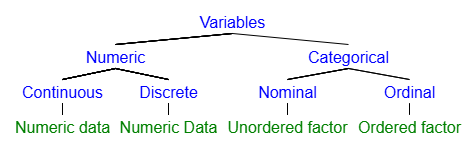
\includegraphics[keepaspectratio]{data_types.png}}

}

\caption{A hierarchy of variables and their corresponding R data types}

\end{figure}%

For our last bit, let's learn a little about working with functions that
don't come included in base R.

\chapter{Packages and the Tidyverse}\label{packages-and-the-tidyverse}

R's open-source culture has encouraged a rich ecosystem of custom
functions designed by scientists and researchers in the R userbase.
These come in the form of `packages', which are suites of several
related functions. For example, there are packages for conducting
statistical tests, producing data visualizations, generating
publication-ready tables, and all manner of other tasks.

\section{Loading Packages}\label{loading-packages}

Let's try this out with one of the better known R packages--`tidyverse'.
This is actually a collection of several packages with a variety of
interrelated functions for `tidying', visualizing, and analyzing data.
We will focus on what we need from `tidyverse', but, if you're curious,
you can read more here: \url{https://www.tidyverse.org/}

If you're on a lab computer, this package may already be installed.
Let's check by running the following command:

\begin{Shaded}
\begin{Highlighting}[]
\FunctionTok{library}\NormalTok{(tidyverse)}
\end{Highlighting}
\end{Shaded}

\begin{verbatim}
-- Attaching core tidyverse packages ------------------------ tidyverse 2.0.0 --
v dplyr     1.1.4     v readr     2.1.5
v forcats   1.0.0     v stringr   1.5.1
v ggplot2   3.5.2     v tibble    3.3.0
v lubridate 1.9.4     v tidyr     1.3.1
v purrr     1.1.0     
-- Conflicts ------------------------------------------ tidyverse_conflicts() --
x dplyr::filter() masks stats::filter()
x dplyr::lag()    masks stats::lag()
i Use the conflicted package (<http://conflicted.r-lib.org/>) to force all conflicts to become errors
\end{verbatim}

If you receive an error when you run this, you likely do not have the
package installed on your system. This is also probably the case if you
are on your personal device and only recently acquired R.

If you got an error, run the following command:

\begin{Shaded}
\begin{Highlighting}[]
\FunctionTok{install.packages}\NormalTok{(}\StringTok{"tidyverse"}\NormalTok{)}
\end{Highlighting}
\end{Shaded}

With a few exceptions, you will always install new packages in this
fashion: install.packages(``package\_name'')

After it's done installing, go back and run the library(tidyverse)
command again. Note that you always need to do this for an added
package. Whether you've had it for a while or just installed it, you
need to load any outside package into your current session by placing
its name in the library() function.

\begin{Shaded}
\begin{Highlighting}[]
\FunctionTok{library}\NormalTok{(tidyverse)}
\end{Highlighting}
\end{Shaded}

\section{Bringing in our Data}\label{bringing-in-our-data}

Let's try bringing in a data frame to play with a few tidyverse
functions. We'll use the \texttt{load()} function to bring in a subset
of the General Social Survey, which contains a few variables from the
2022 survey wave. Run the following command and select the file
``our\_gss.rda''

\begin{Shaded}
\begin{Highlighting}[]
\FunctionTok{load}\NormalTok{(}\FunctionTok{file.choose}\NormalTok{())}
\end{Highlighting}
\end{Shaded}

The \texttt{file.choose()} function will open up a file-explorer window
that allows you to manually select an R data file to load in. We'll talk
about some other ways to import data files using R syntax next time.

Go ahead and take a look at the data frame. Each GSS survey wave has
about 600-700 variables in total, so I've plucked several and done a
little pre-processing to get us a subset to work with. All the variables
here have pretty straightforward names, but I'll note that
\texttt{realrinc} is a clear outlier there. This is short for `Real
respondent's income' and reflects the respondent's income reported in
exact dollar amounts. I'll put a summary here so you can take a look if
you're not following along with your own script.

\begin{Shaded}
\begin{Highlighting}[]
\FunctionTok{summary}\NormalTok{(our\_gss)}
\end{Highlighting}
\end{Shaded}

\begin{verbatim}
      year            id              age           race          sex      
 Min.   :2022   Min.   :   1.0   Min.   :18.00   black: 565   female:1897  
 1st Qu.:2022   1st Qu.: 886.8   1st Qu.:34.00   other: 412   male  :1627  
 Median :2022   Median :1772.5   Median :48.00   white:2514   NA's  :  20  
 Mean   :2022   Mean   :1772.5   Mean   :49.18   NA's :  53                
 3rd Qu.:2022   3rd Qu.:2658.2   3rd Qu.:64.00                             
 Max.   :2022   Max.   :3545.0   Max.   :89.00                             
                                 NA's   :208                               
    realrinc                        educ    
 Min.   :   204.5   12th grade        :909  
 1st Qu.:  8691.2   4 years of college:697  
 Median : 18405.0   2 years of college:506  
 Mean   : 27835.3   1 year of college :268  
 3rd Qu.: 33742.5   6 years of college:210  
 Max.   :141848.3   (Other)           :934  
 NA's   :1554       NA's              : 20  
                               partyid   
 independent (neither, no response):835  
 strong democrat                   :595  
 not very strong democrat          :451  
 strong republican                 :431  
 independent, close to democrat    :400  
 (Other)                           :797  
 NA's                              : 35  
\end{verbatim}

\section{Data Wrangling with
Tidyverse}\label{data-wrangling-with-tidyverse}

Let's use this subset to explore some tidyverse functionality. Tidyverse
includes several functions for efficiently manipulating data frames in
preparation for analyses. We will encounter a number of these throughout
our time with R, but I want to briefly introduce a few key functions and
operations that we will dig into more next time.

\subsection{select()}\label{select}

It happens quite often that we have a data frame containing far more
variables than we ultimately need for a given analysis. The
\texttt{select()} function allows us to quickly subset data frames
according to the variable columns we need.

\begin{Shaded}
\begin{Highlighting}[]
\NormalTok{sex\_inc }\OtherTok{\textless{}{-}} \FunctionTok{select}\NormalTok{(our\_gss, id, sex, realrinc)}
\end{Highlighting}
\end{Shaded}

You should now have an object that contains all 3,544 observations, but
includes only the 3 columns that we specified with \texttt{select()}.

\begin{Shaded}
\begin{Highlighting}[]
\FunctionTok{summary}\NormalTok{(sex\_inc)}
\end{Highlighting}
\end{Shaded}

\begin{verbatim}
       id             sex          realrinc       
 Min.   :   1.0   female:1897   Min.   :   204.5  
 1st Qu.: 886.8   male  :1627   1st Qu.:  8691.2  
 Median :1772.5   NA's  :  20   Median : 18405.0  
 Mean   :1772.5                 Mean   : 27835.3  
 3rd Qu.:2658.2                 3rd Qu.: 33742.5  
 Max.   :3545.0                 Max.   :141848.3  
                                NA's   :1554      
\end{verbatim}

\subsection{filter()}\label{filter}

\texttt{filter()} functions similarly except that, instead of
sub-setting by specific variables, it allows you to subset by specific
values. So, let's take the \texttt{sex\_inc} object we just created
above. We now have this subset of three variables---id, sex, and
income---but let's imagine we want to answer a question that's specific
to women.

In order to do that, we need to \emph{filter} the data to include only
observations where the value of the variable \texttt{sex} is `female'.

\begin{Shaded}
\begin{Highlighting}[]
\NormalTok{fem\_inc }\OtherTok{\textless{}{-}} \FunctionTok{filter}\NormalTok{(sex\_inc, sex}\SpecialCharTok{==}\StringTok{"female"}\NormalTok{)}
\end{Highlighting}
\end{Shaded}

Note that the \texttt{fem\_inc} object still has 3 variables, but there
are now roughly half the observations, suggesting that we have
successfully filtered out the male observations.

\begin{Shaded}
\begin{Highlighting}[]
\FunctionTok{summary}\NormalTok{(fem\_inc)}
\end{Highlighting}
\end{Shaded}

\begin{verbatim}
       id           sex          realrinc       
 Min.   :   1   female:1897   Min.   :   204.5  
 1st Qu.: 879   male  :   0   1st Qu.:  7668.8  
 Median :1783                 Median : 15337.5  
 Mean   :1772                 Mean   : 22702.1  
 3rd Qu.:2664                 3rd Qu.: 27607.5  
 Max.   :3544                 Max.   :141848.3  
                              NA's   :883       
\end{verbatim}

\subsection{summarize()}\label{summarize}

As the name suggests, \texttt{summarize()} allows us to quickly
summarize information across variables. It will give us a new data frame
that reflects the particular summaries that we ask for, which can be
very useful for quickly generating means within and across different
variables.

Let's try another simple use case, and then I'll introduce a concept
that will help us learn to chain these functions together.

\begin{Shaded}
\begin{Highlighting}[]
\NormalTok{mean\_inc }\OtherTok{\textless{}{-}} \FunctionTok{summarize}\NormalTok{(our\_gss, }\StringTok{"mean\_inc"}\OtherTok{=}\FunctionTok{mean}\NormalTok{(realrinc, }\AttributeTok{na.rm=}\ConstantTok{TRUE}\NormalTok{))}
\end{Highlighting}
\end{Shaded}

\begin{tcolorbox}[enhanced jigsaw, colback=white, title=\textcolor{quarto-callout-note-color}{\faInfo}\hspace{0.5em}{Note}, coltitle=black, bottomrule=.15mm, breakable, opacityback=0, colframe=quarto-callout-note-color-frame, leftrule=.75mm, opacitybacktitle=0.6, arc=.35mm, rightrule=.15mm, bottomtitle=1mm, toptitle=1mm, titlerule=0mm, toprule=.15mm, left=2mm, colbacktitle=quarto-callout-note-color!10!white]

You probably noticed the \texttt{na.rm\ =\ TRUE} input that I supplied
for the above function. This is short for `remove NAs', which we need to
do when a variable has any NA values. If we don't, R will return an
error, because it does not know to disregard NA values when calculating
a column mean.

\end{tcolorbox}

This gives us a new data frame that we called \texttt{mean\_inc}. It
should have 1 row and 1 column, and it just gives us the average income
of a person in our GSS subset---about \$28,000/year.

\begin{Shaded}
\begin{Highlighting}[]
\NormalTok{mean\_inc}
\end{Highlighting}
\end{Shaded}

\begin{verbatim}
  mean_inc
1 27835.33
\end{verbatim}

Now, this is not really all that impressive when we are asking for a
broad summary like this. In fact, if all we wanted was to see the
average income, we could get that more easily, e.g.

\begin{Shaded}
\begin{Highlighting}[]
\FunctionTok{mean}\NormalTok{(our\_gss}\SpecialCharTok{$}\NormalTok{realrinc, }\AttributeTok{na.rm =} \ConstantTok{TRUE}\NormalTok{)}
\end{Highlighting}
\end{Shaded}

\begin{verbatim}
[1] 27835.33
\end{verbatim}

The true power of \texttt{summarize()} comes from chaining it together
with other tidyverse functions. However, in order to do that, we will
need to learn about one more new R operation.

\section{The Pipe}\label{the-pipe}

This one might be a little unintuitive, so don't worry if it doesn't
immediately click. We will continue to get plenty of practice with it
over the next couple of sessions.

The pipe operator looks like this: \texttt{\textbar{}\textgreater{}}.
What it does is take whatever is to the left of the symbol and `pipe' it
into the function on the right-hand side. That probably sounds a little
strange, so let's see some examples.

We'll refer back to our \texttt{summarize()} command from above.

\begin{Shaded}
\begin{Highlighting}[]
\NormalTok{mean\_inc }\OtherTok{\textless{}{-}} \FunctionTok{summarize}\NormalTok{(our\_gss, }\StringTok{"mean\_inc"}\OtherTok{=}\FunctionTok{mean}\NormalTok{(realrinc, }\AttributeTok{na.rm=}\ConstantTok{TRUE}\NormalTok{))}
\end{Highlighting}
\end{Shaded}

This is equivalent to\ldots{}

\begin{Shaded}
\begin{Highlighting}[]
\NormalTok{mean\_inc }\OtherTok{\textless{}{-}}\NormalTok{ our\_gss }\SpecialCharTok{|\textgreater{}}
  \FunctionTok{summarize}\NormalTok{(}\StringTok{"mean\_age"} \OtherTok{=} \FunctionTok{mean}\NormalTok{(realrinc, }\AttributeTok{na.rm=}\ConstantTok{TRUE}\NormalTok{))}
\end{Highlighting}
\end{Shaded}

Notice that, in the first command, the first input that we give
\texttt{summarize()} is the data frame that we want it to work with.

In the command featuring the pipe operator, we supply the data frame and
then pipe it into \texttt{summarize()}. The real magic comes from
chaining multiple pipes together. This will likely take a little
practice to get used to, but it can become a very powerful tool in our R
arsenal.

\subsection{Putting It All Together}\label{putting-it-all-together}

Let's illustrate with an example. I'll let you know what I want to do in
plain English, and then I will execute that desire with multiple piped
commands.

Ultimately, I want to see the mean income, but I want to see the mean
broken down by sex rather than the mean of the entire data frame.

So, I want to take a \textbf{selection} of variables from
\texttt{our\_gss}. I want these variables to be \textbf{grouped by}
\texttt{sex}. Finally, I want to see a \textbf{summary} of the mean
according to this variable grouping.

\begin{Shaded}
\begin{Highlighting}[]
\NormalTok{sex\_means }\OtherTok{\textless{}{-}}\NormalTok{ our\_gss }\SpecialCharTok{|\textgreater{}}
  \FunctionTok{select}\NormalTok{(id, sex, realrinc) }\SpecialCharTok{|\textgreater{}}
  \FunctionTok{group\_by}\NormalTok{(sex) }\SpecialCharTok{|\textgreater{}}
  \FunctionTok{summarize}\NormalTok{(}\StringTok{"mean\_inc"} \OtherTok{=} \FunctionTok{mean}\NormalTok{(realrinc, }\AttributeTok{na.rm=}\ConstantTok{TRUE}\NormalTok{))}
\end{Highlighting}
\end{Shaded}

\begin{tcolorbox}[enhanced jigsaw, colback=white, title=\textcolor{quarto-callout-note-color}{\faInfo}\hspace{0.5em}{Note}, coltitle=black, bottomrule=.15mm, breakable, opacityback=0, colframe=quarto-callout-note-color-frame, leftrule=.75mm, opacitybacktitle=0.6, arc=.35mm, rightrule=.15mm, bottomtitle=1mm, toptitle=1mm, titlerule=0mm, toprule=.15mm, left=2mm, colbacktitle=quarto-callout-note-color!10!white]

Note that I've added one new function here, \texttt{group\_by()}. We'll
see this plenty more in other cases, and it will help us quite a bit
when it comes to summary statistics. As the name suggests, it applies a
grouping structure that can be leveraged with all kinds of other
functions.

\end{tcolorbox}

\begin{Shaded}
\begin{Highlighting}[]
\NormalTok{sex\_means}
\end{Highlighting}
\end{Shaded}

\begin{verbatim}
# A tibble: 3 x 2
  sex    mean_inc
  <fct>     <dbl>
1 female   22702.
2 male     33191.
3 <NA>     11248.
\end{verbatim}

Notice that this will give us a new data frame with the average income
of \texttt{sex} for both \texttt{male} and \texttt{female}. However, we
actually get a 3rd row for NAs, which is a 3rd category of the
\texttt{sex} variable. At the level of the survey, it's important to
keep track of this for a number of reasons, but we do not need them for
our purposes. So, we can add a final pipe with the \texttt{drop\_na()}
function in order to drop the NA level of \texttt{sex}.

\begin{Shaded}
\begin{Highlighting}[]
\NormalTok{sex\_means }\OtherTok{\textless{}{-}}\NormalTok{ our\_gss }\SpecialCharTok{|\textgreater{}}
  \FunctionTok{select}\NormalTok{(id, sex, realrinc) }\SpecialCharTok{|\textgreater{}}
  \FunctionTok{group\_by}\NormalTok{(sex) }\SpecialCharTok{|\textgreater{}}
  \FunctionTok{summarize}\NormalTok{(}\StringTok{"mean\_inc"} \OtherTok{=} \FunctionTok{mean}\NormalTok{(realrinc, }\AttributeTok{na.rm=}\ConstantTok{TRUE}\NormalTok{)) }\SpecialCharTok{|\textgreater{}}
  \FunctionTok{drop\_na}\NormalTok{(sex)}

\NormalTok{sex\_means}
\end{Highlighting}
\end{Shaded}

\begin{verbatim}
# A tibble: 2 x 2
  sex    mean_inc
  <fct>     <dbl>
1 female   22702.
2 male     33191.
\end{verbatim}

We will see plenty more on the tidyverse, so don't fret if these new
functions are not completely clicking right away. We will keep building
with these in the next unit and hopefully accumulate some muscle memory.

\chapter{Word Embeddings with US Federal Job
Advertisements}\label{word-embeddings-with-us-federal-job-advertisements}

The following code reproduces components of the analysis for the
in-progress manuscript, ``Occupational Segregation and Gendered Language
in Job Advertisements''

This project investigates whether and to what extent the gendered
composition of the federal workforce is associated with the amount of
gender stereotypical language in federal job advertisements, and, if so,
whether this relationship holds across different organizational
climates.

Our data comprises 5,526 job ads scraped at a single timepoint from the
US federal job-posting site USAJobs.gov, along with a number of
occupational characteristics imported from other sources such as the
Current Population Survey, O*NET, The Federal Employee Viewpoint Survey,
and the Survey on the Future of Government Service.

We conceptualize stereotype language in terms of social psycholoy's
Stereotype Content Model
\href{https://www.sciencedirect.com/science/article/pii/S0065260107000020?casa_token=HABSzi8Y7JMAAAAA:LBi45HX4KWxLfP4LLjsP8ySkpW1JtcZBNl67r55dZjmKbzsggVNarS--N6Y9XWdcn_q3zGfTI_c}{(Cuddy,
Fiske, and Glick 2008)}. To operationalize the stereotype content model,
we utilized word embeddings in conjunction with
\href{https://link.springer.com/article/10.1007/s42001-019-00048-6}{Stoltz
and Taylor's (2019)} Concept Mover's Distance as an instrument for
measuring the degree of warmth- and competence-language across job ads.

\section{Setting up the Workspace}\label{setting-up-the-workspace}

Let's load some packages

\begin{verbatim}
Skipping install of 'text2map.pretrained' from a gitlab remote, the SHA1 (f17fbff7) has not changed since last install.
  Use `force = TRUE` to force installation
\end{verbatim}

\begin{Shaded}
\begin{Highlighting}[]
\FunctionTok{library}\NormalTok{(ggrepel)}
\FunctionTok{library}\NormalTok{(text2map)}
\FunctionTok{library}\NormalTok{(text2vec)}
\FunctionTok{library}\NormalTok{(gutenbergr)}
\FunctionTok{library}\NormalTok{(tidyverse)}
\FunctionTok{library}\NormalTok{(textclean)}
\FunctionTok{library}\NormalTok{(stringi)}
\FunctionTok{library}\NormalTok{(text2map.pretrained)}
\FunctionTok{library}\NormalTok{(flextable)}
\FunctionTok{library}\NormalTok{(huxtable)}
\FunctionTok{library}\NormalTok{(sjPlot)}
\FunctionTok{library}\NormalTok{(interactions)}
\FunctionTok{library}\NormalTok{(remotes)}
\end{Highlighting}
\end{Shaded}

You might have to install a couple of these, but all of them can be
installed with \texttt{install.packages()} except for
\texttt{text2map.pretrained}, so go ahead and download that with the
following command

\begin{Shaded}
\begin{Highlighting}[]
\NormalTok{remotes}\SpecialCharTok{::}\FunctionTok{install\_gitlab}\NormalTok{(}\StringTok{"culturalcartography/text2map.pretrained"}\NormalTok{)}
\end{Highlighting}
\end{Shaded}

Now, go ahead and load ``workingjobs.df'' into your workspace. You can
use \texttt{file.choose()} with \texttt{load()} to pull up a
file-explorer window and manually select the data.

\begin{Shaded}
\begin{Highlighting}[]
\FunctionTok{load}\NormalTok{(}\FunctionTok{file.choose}\NormalTok{())}
\end{Highlighting}
\end{Shaded}

We also need to download our pre-trained vector embeddings. We use
\href{https://fasttext.cc/docs/en/english-vectors.html}{fastText
embeddings}, which are trained on a large corpus of English Wikipedia
and various news data sets. This way, our embeddings will reflect a
sense of public meaning. This works well for many research questions,
but you may want to consider training your own embeddings in the event
that your data is stylistically unique.

\begin{tcolorbox}[enhanced jigsaw, colback=white, title=\textcolor{quarto-callout-caution-color}{\faFire}\hspace{0.5em}{Caution}, coltitle=black, bottomrule=.15mm, breakable, opacityback=0, colframe=quarto-callout-caution-color-frame, leftrule=.75mm, opacitybacktitle=0.6, arc=.35mm, rightrule=.15mm, bottomtitle=1mm, toptitle=1mm, titlerule=0mm, toprule=.15mm, left=2mm, colbacktitle=quarto-callout-caution-color!10!white]

The fastText embeddings file is very large. It will be over a gigabyte,
so keep that in mind before you download. You only have to run the
following command once ever, so consider commenting it out of your
script after you do so. You don't want to keep downloading such a huge
file by mistake.

\end{tcolorbox}

\begin{Shaded}
\begin{Highlighting}[]
\FunctionTok{download\_pretrained}\NormalTok{(}\StringTok{"vecs\_fasttext300\_wiki\_news"}\NormalTok{)}
\end{Highlighting}
\end{Shaded}

After that finishes downloading, go ahead and load the embeddings object
in. You will want to do this anytime you work with your embeddings. It
won't download anything new---it just retrieves the file you downloaded
with the command above.

\begin{Shaded}
\begin{Highlighting}[]
\FunctionTok{data}\NormalTok{(}\StringTok{"vecs\_fasttext300\_wiki\_news"}\NormalTok{)}
\NormalTok{our\_wv}\OtherTok{\textless{}{-}}\NormalTok{vecs\_fasttext300\_wiki\_news}
\FunctionTok{rm}\NormalTok{(vecs\_fasttext300\_wiki\_news)}
\end{Highlighting}
\end{Shaded}

Because the file name is a bit cumbersome, Stoltz \& Taylor recommend
renaming the object and then removing the original file.

\section{Calculating our Response Variable with Concept Mover's
Distance}\label{calculating-our-response-variable-with-concept-movers-distance}

Below, we will use pre-trained vector encodings to calculate the Concept
Mover's Distance for stereotype content language across all of our job
ads. Note that much of this section makes heavy use of the excellent
\href{https://culturalcartography.gitlab.io/text2map/}{text2map} package
from
\href{https://global.oup.com/academic/product/mapping-texts-9780197756881?cc=us&lang=en&}{Stoltz
and Taylor (2023)}.

\subsection{Wrangle our Embeddings}\label{wrangle-our-embeddings}

First, we'll borrow some code from \emph{Mapping Texts} to build a
document-term matrix. This will give us a new dataframe where each row
is a document, each column is a single word, and each cell reflects the
count of some word in a given document.

\begin{Shaded}
\begin{Highlighting}[]
\NormalTok{dtm\_ja }\OtherTok{\textless{}{-}}\NormalTok{ workingjobs.df }\SpecialCharTok{|\textgreater{}}
  \FunctionTok{dtm\_builder}\NormalTok{(string\_lemma, doc\_id) }\SpecialCharTok{|\textgreater{}}
  \FunctionTok{dtm\_stopper}\NormalTok{(}\AttributeTok{stop\_list =} \FunctionTok{get\_stoplist}\NormalTok{(}\StringTok{"snowball2014"}\NormalTok{),}
              \AttributeTok{stop\_docprop =} \FunctionTok{c}\NormalTok{(.}\DecValTok{01}\NormalTok{, }\ConstantTok{Inf}\NormalTok{))}
\end{Highlighting}
\end{Shaded}

\texttt{string\_lemma} is the column that contains our job ad text after
various pre-processing procedures. Note that we are also removing a list
of common stop words, using the predefined Snowball list. Stop words are
typically function words that occur with high frequency. For cultural
measurement of text data, we are often more interested in content words
that bare more straightforward semantic information, so including stop
words can muddy our instrument. Lastly, we use \texttt{stop\_docprop} to
set a low-end exclusion criteria for word frequency. Any word that
appears in less than 1\% of all documents will be dropped from our DTM.

Now, let's take a subset of the word embeddings object. We want an
object that includes the vector embeddings for only the words in our
cleaned DTM. Remember that the columns of the DTM are words in the job
ads corpus, and the row names of \texttt{our\_wv} are all 1 million
words in the pre-trained embeddings. We can use this to subset.

\begin{Shaded}
\begin{Highlighting}[]
\NormalTok{job\_vectors }\OtherTok{\textless{}{-}}\NormalTok{ our\_wv[}\FunctionTok{rownames}\NormalTok{(our\_wv) }\SpecialCharTok{\%in\%} \FunctionTok{colnames}\NormalTok{(dtm\_ja), ]}
\end{Highlighting}
\end{Shaded}

\subsection{Mapping Warmth and
Competence}\label{mapping-warmth-and-competence}

For Concept Mover's Distance, we need two word lists reflecting each of
our two oppositional concepts of interest. Let's load in our paired
lists of warmth and competence words. Note that we derived these pairs
from the warmth/competence seed dictionary created by
\href{https://onlinelibrary.wiley.com/doi/full/10.1002/ejsp.2724?casa_token=gqMHBVmq7eUAAAAA\%3Azr6pilqgfE2nbpJ6yt1aikGXx4GZnenVpTp3F6g9kEPglQqBvFedzgMtbFPuH0mVQ1JUUkzgitZeR6M}{Gandalf,
Bai, and Fiske's (2020)}.

\begin{Shaded}
\begin{Highlighting}[]
\FunctionTok{load}\NormalTok{(}\FunctionTok{file.choose}\NormalTok{())}
\end{Highlighting}
\end{Shaded}

Go ahead and load in ``scm\_antonym\_pairs.csv''

Now we will calculate a semantic direction using our paired wordlist and
our original word embedding object, \texttt{our\_wv}. The semantic
direction is the difference of the two vectors, which gives us the pole
between the warmth and competence regions we defined in embedding space.

Then, we'll use the semantic direction to generate the Concept Mover's
Distance for each job. You can refer to Stoltz \& Taylor's original
paper on this for more details on the calculation, but it essentially
maps each document along the semantic direction pole. This will allow us
to estimate how close the vector space of each job ad is to the
competence region vs.~the warmth region. This gives us our measure of
conceptual prominence.

\begin{Shaded}
\begin{Highlighting}[]
\NormalTok{sd\_stereo }\OtherTok{\textless{}{-}} \FunctionTok{get\_direction}\NormalTok{(scm\_ant, our\_wv, }\AttributeTok{method=}\StringTok{"paired"}\NormalTok{)}
\NormalTok{closeness }\OtherTok{\textless{}{-}} \FunctionTok{CMDist}\NormalTok{(}\AttributeTok{dtm=}\NormalTok{ dtm\_ja, }\AttributeTok{cv =}\NormalTok{ sd\_stereo, }\AttributeTok{wv =}\NormalTok{ job\_vectors)}
\end{Highlighting}
\end{Shaded}

The \texttt{closeness} object will be a 2-column data frame including
the Concept Mover's Distance scores for each ad and the \texttt{doc\_id}
column, which we can use to merge these values into our job ads data
frame.

Because of the way we set up our paired wordlist, positive values
reflect more engagement with competence language, and negative values
reflect more warmth engagement.

Note that it will name the CMD column with the format \texttt{*\_pole},
where \texttt{*} is a stand-in for the first word on the left-side of
our wordlist of warmth/competence pairs. That will be `ability' in our
case, so let's rename it something more descriptive.

\begin{Shaded}
\begin{Highlighting}[]
\FunctionTok{names}\NormalTok{(closeness)[}\DecValTok{2}\NormalTok{]}\OtherTok{\textless{}{-}}\StringTok{"comp\_warm\_scale"}
\end{Highlighting}
\end{Shaded}

Now, we can merge these values into our original data frame.

\begin{Shaded}
\begin{Highlighting}[]
\NormalTok{workingjobs.df }\OtherTok{\textless{}{-}} \FunctionTok{merge}\NormalTok{(workingjobs.df, closeness)}
\end{Highlighting}
\end{Shaded}

\subsection{View the Warmest and Most Competence
Words}\label{view-the-warmest-and-most-competence-words}

Now we've got our measure of warmth/competence prominence! There's
plenty more we can do with embeddings, but we are winding down the
current tutorial.

I'll leave you with one last neat example highlighted in \emph{Mapping
Texts} I will borrow some more code from Stoltz and Taylor to show you
how you can view the individual words whose vector embeddings were
closest to warmth or competence. CMD is a document level measure, but we
can do all kinds of fun stuff with individual embeddings. Below are the
words estimated to most strongly engage one concept or the other.

\begin{Shaded}
\begin{Highlighting}[]
\NormalTok{comp\_warm }\OtherTok{\textless{}{-}} \FunctionTok{get\_direction}\NormalTok{(}\AttributeTok{anchors =}\NormalTok{ scm\_ant, }\AttributeTok{wv =}\NormalTok{ our\_wv, }\AttributeTok{method=}\StringTok{"paired"}\NormalTok{)}

\FunctionTok{row.names}\NormalTok{(comp\_warm)[}\DecValTok{1}\NormalTok{]}\OtherTok{\textless{}{-}}\StringTok{"competence\_pole"}

\NormalTok{sim\_dir }\OtherTok{\textless{}{-}} \FunctionTok{sim2}\NormalTok{(comp\_warm, job\_vectors, }\AttributeTok{method =} \StringTok{"cosine"}\NormalTok{)}
\NormalTok{df\_dir }\OtherTok{\textless{}{-}} \FunctionTok{data.frame}\NormalTok{(}\AttributeTok{competence\_pole =}\NormalTok{ sim\_dir[}\StringTok{"competence\_pole"}\NormalTok{, ],}
                     \AttributeTok{terms =} \FunctionTok{colnames}\NormalTok{(sim\_dir)) }\SpecialCharTok{|\textgreater{}}
  \FunctionTok{mutate}\NormalTok{(}\AttributeTok{comp\_warm\_label =} \FunctionTok{ifelse}\NormalTok{(}
\NormalTok{    competence\_pole }\SpecialCharTok{\textgreater{}=} \DecValTok{0}\NormalTok{,}
    \StringTok{"Competence"}\NormalTok{, }\StringTok{"Warmth"}\NormalTok{),}
    \AttributeTok{comp\_warm =} \FunctionTok{abs}\NormalTok{(competence\_pole)}
\NormalTok{  )}

\NormalTok{df\_dir }\SpecialCharTok{|\textgreater{}}
  \FunctionTok{group\_by}\NormalTok{(comp\_warm\_label) }\SpecialCharTok{|\textgreater{}}
  \FunctionTok{slice\_max}\NormalTok{(comp\_warm, }\AttributeTok{n =} \DecValTok{30}\NormalTok{) }\SpecialCharTok{|\textgreater{}}
  \FunctionTok{mutate}\NormalTok{(}\AttributeTok{term =} \FunctionTok{fct\_reorder}\NormalTok{(terms, comp\_warm)) }\SpecialCharTok{|\textgreater{}}
  \FunctionTok{ggplot}\NormalTok{(}\FunctionTok{aes}\NormalTok{(term, comp\_warm, }\AttributeTok{fill =}\NormalTok{ comp\_warm\_label, }\AttributeTok{label =}\NormalTok{ terms)) }\SpecialCharTok{+}
  \FunctionTok{geom\_col}\NormalTok{() }\SpecialCharTok{+}
  \FunctionTok{guides}\NormalTok{(}\AttributeTok{fill =} \StringTok{"none"}\NormalTok{) }\SpecialCharTok{+}
  \FunctionTok{labs}\NormalTok{(}\AttributeTok{x =} \ConstantTok{NULL}\NormalTok{, }\AttributeTok{y =} \StringTok{"Cosine Similarity to Pole"}\NormalTok{) }\SpecialCharTok{+}
  \FunctionTok{coord\_flip}\NormalTok{() }\SpecialCharTok{+}
  \FunctionTok{facet\_wrap}\NormalTok{(}\SpecialCharTok{\textasciitilde{}}\NormalTok{comp\_warm\_label, }\AttributeTok{scale =} \StringTok{"free"}\NormalTok{)}
\end{Highlighting}
\end{Shaded}

\pandocbounded{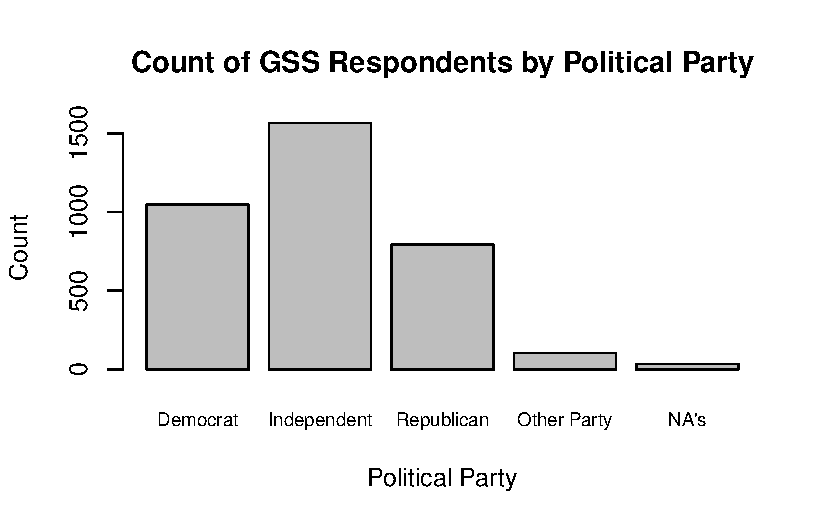
\includegraphics[keepaspectratio]{usajobs_embeddings_files/figure-pdf/unnamed-chunk-15-1.pdf}}

\part{Day 2: Survey Data and Univariate Analysis}

\part{Day 3: Bivariate Analysis with the GSS}

\part{Day 4: Multivariable Analysis and Elaboration}

\part{Day 5: Data Visualization and ggplot}

\chapter*{Introduction}\label{introduction}
\addcontentsline{toc}{chapter}{Introduction}

\markboth{Introduction}{Introduction}

Up to this point, we have worked with pretty simple visualizations, just
so we can quickly glean important information about our statistical
models without spending too much time focusing on the aesthetics of the
visuals.

In this lab, we will learn a bit more about R's graphical
capability---especially through tidyverse's \texttt{ggplot}---which
provides us with incredible customizability. We will learn how to
fine-tune some of the visuals we have already worked with, and we will
preview some other common visual styles that can manage with
\texttt{ggplot}.

\section*{Visualization and Analytical
Thinking}\label{visualization-and-analytical-thinking}
\addcontentsline{toc}{section}{Visualization and Analytical Thinking}

\markright{Visualization and Analytical Thinking}

Before we start working with some of these new visual tools, I want to
take an opportunity to stress the importance of visualization more
generally. It's easy to see the process of presenting visuals as
something somewhat superficial, but visualization can be critical for
defining the kind of questions we can ask about our data.

For now, I'm going to obscure the code I'm using for this document. We
will learn more about the kind of commands I used to generate the
following figures, but I don't want anyone to get bogged down initially.
I'll use these visuals to help impart an important lesson about data
visualization's in the research process.

\section*{Thirteen Data Sets}\label{thirteen-data-sets}
\addcontentsline{toc}{section}{Thirteen Data Sets}

\markright{Thirteen Data Sets}

Let's take a look at a collection of thirteen different data sets. Each
data set has 142 observations with 2 columns, labeled x \& y.

I'll use some tidyverse commands to get some summary statistics for each
of the data sets, including the mean of both variables and their
standard deviations. Let's see what seems to distinguish some of these
data sets from one another.

\begin{verbatim}
# A tibble: 13 x 4
   mean_x mean_y std_x std_y
    <dbl>  <dbl> <dbl> <dbl>
 1   54.3   47.8  16.8  26.9
 2   54.3   47.8  16.8  26.9
 3   54.3   47.8  16.8  26.9
 4   54.3   47.8  16.8  26.9
 5   54.3   47.8  16.8  26.9
 6   54.3   47.8  16.8  26.9
 7   54.3   47.8  16.8  26.9
 8   54.3   47.8  16.8  26.9
 9   54.3   47.8  16.8  26.9
10   54.3   47.8  16.8  26.9
11   54.3   47.8  16.8  26.9
12   54.3   47.8  16.8  26.9
13   54.3   47.8  16.8  26.9
\end{verbatim}

Well, there's not much we can say here. All the summary statistics are
identical. Why don't we try modeling a linear relationship between the x
and y variables. Maybe looking at the correlations will tell us
something. I'll display the linear regression lines for each data set
below.

\pandocbounded{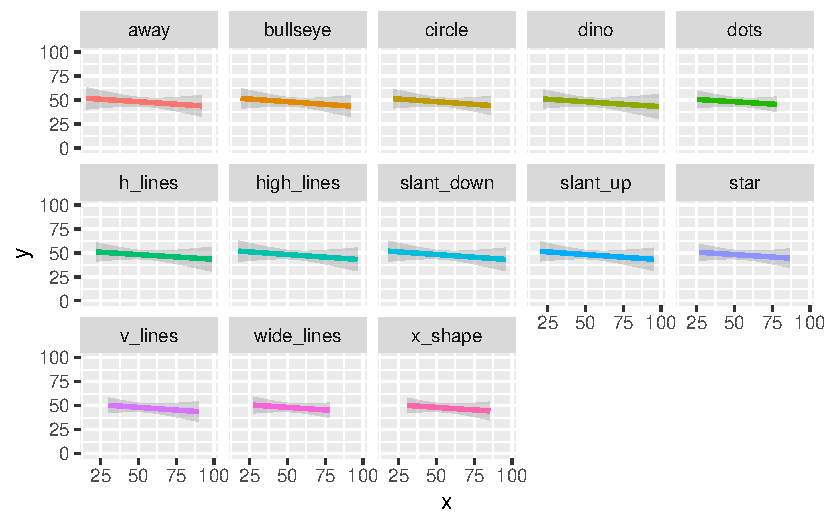
\includegraphics[keepaspectratio]{viz_introduction_files/figure-pdf/unnamed-chunk-2-1.pdf}}

Okay. This is not revealing much either. All the lines seem to have the
same slope, which shows a (slight) negative relationship where y
decreases as x increases. The correlations aren't revealing any notable
distinctions.

But wait. One thing we can see here is that, while the correlations
appear to be about the same, there are some differences in the ranges of
values. Note that the regression lines don't extend across the same
range of x-axis values in each data set. Maybe there is something here
after all.

Let's just go ahead and plot the actual data over our regression lines.

\pandocbounded{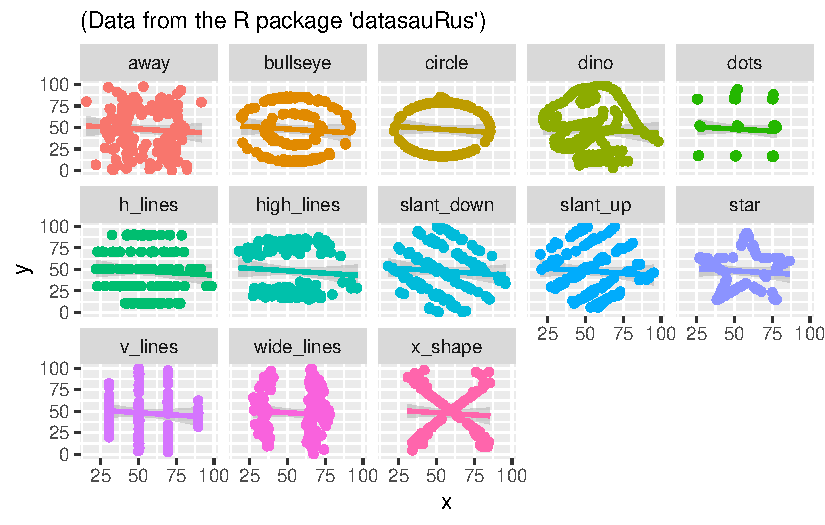
\includegraphics[keepaspectratio]{viz_introduction_files/figure-pdf/unnamed-chunk-3-1.pdf}}

Now there's some distinction!

This is a tongue in cheek data set known as the
\href{https://jumpingrivers.github.io/datasauRus/}{`datasaurus dozen'}.
It's often used in intro statistical classes to help illustrate the
importance of visualization. It's inspired by another conceptually
similar data set known as
\href{https://en.wikipedia.org/wiki/Anscombe\%27s_quartet}{`Anscombe's
quartet'} which likewise stresses the role of plotting data in producing
well informed analyses.

\section*{In Sum}\label{in-sum}
\addcontentsline{toc}{section}{In Sum}

\markright{In Sum}

So, take this as a showcase of the importance of visualizing your data.
This isn't to discount summary statistics and other numeric description
of data---those are still invaluable for us.

Rather, cases like Datasaurus or Anscombe's quartet highlight the
necessity of understanding the shape of your data. This will determine
the kind of questions you can ask with the data, as well as the kind of
statistical tools you need to describe it.

For example, in the case we just examined, those x and y variables do
not have any kind of clear linear relationship. In that case, tools like
regression that assume linearity are not appropriate. Any relationship
between the variables could only be explored through other statistical
means.

So, making our figures and tables look aesthetically pleasing is indeed
valuable in its own right, but don't underestimate the utility of good
visualization for the analytic process itself.




\end{document}
